% This is a model template for the solutions in computational science. You can find a very useful documentation for LaTeX in Finnish at ftp://ftp.funet.fi/pub/TeX/CTAN/info/lshort/finnish/ or in English at ftp://ftp.funet.fi/pub/TeX/CTAN/info/lshort/english/. The section List of mathematical symbols in Chapter 3 is especially useful for the typesetting of mathematical formulas.

% Compile the document to PDF by command 'pdflatex model.tex' in the terminal. The command must be run twice for the references in the text to be correct.

\documentclass[a4paper,11pt]{article}
\usepackage[utf8]{inputenc}
% This includes letters such as � and �
\usepackage[T1]{fontenc}
% Use here 'Finnish' for Finnish hyphenation. You may have to compile the code twice after the change. 
\usepackage[english]{babel}
\usepackage{graphicx}
% Some math stuff
\usepackage{amsmath,amsfonts,amssymb,amsbsy,commath,booktabs,hyperref}  
% This is just to include the urls
\usepackage{hyperref}
\usepackage[margin=2cm]{geometry}

\setlength{\parindent}{0mm}
\setlength{\parskip}{1.0\baselineskip}

\usepackage{listings}
\usepackage{color}

\definecolor{dkgreen}{rgb}{0,0.6,0}
\definecolor{gray}{rgb}{0.5,0.5,0.5}
\definecolor{mauve}{rgb}{0.58,0,0.82}

\lstset{frame=tb,
	language=Python,
	aboveskip=3mm,
	belowskip=3mm,
	showstringspaces=false,
	columns=flexible,
	basicstyle={\small\ttfamily},
	numbers=none,
	numberstyle=\tiny\color{gray},
	keywordstyle=\color{blue},
	commentstyle=\color{dkgreen},
	stringstyle=\color{mauve},
	breaklines=true,
	breakatwhitespace=true,
	tabsize=4
}

\begin{document}

\title{Becs-114.1100 Computational Science -- exercise round 3} % Replace the exercise round number
\author{Kunal Ghosh, 546247} % Replace with your name and student number
\maketitle
\section{Solution to Question 3 (a)}\label{prob3a}

In this problem we need to compute how well a particular polynomial can interpolate a given set of data. We will also discover the effect of interpolating points on the final interpolation by the same degree polynomial.

For the first part we are required to choose 13 equally spaced points on the given polynomial $\frac{x}{\frac{1}{4} + x^2}$ The 13 chosen points have been plotted as the blue dots on \ref{fig:fig1} and a 12 degree polynomial has been interpolated as can be seen as the red line passing through all the 13 interpolating points.

However, it can be seen in \ref{fig:err1} that the interpolated function has large errors on either end. This results in increasing the overall mean absolute error between the target function and the interpolating function, which in this case is 0.137122949967.

Note:
I was just curious to figure out the reason behind higher order polynomials oscillating wildly as n ( the distance from 0 on the x axis ). Apparently that's because of Runge's phenomenon (\url{https://en.wikipedia.org/wiki/Runge's_phenomenon}) which just boils down to. I did not fully understand the lebesgue constant part. But the first point of derivatives of higher order functions increasing rapidly with increasing values of x. This essentially means, that higher order functions would be more wavy if not controlled by more interpolating points , as x grows. This is exactly what we see in this section and the next.

Any suggestions / comments that might help clear any misconceptions I might have or which might help me understand the concept better, are welcome !
 
	
\begin{figure}[h]
	\center
	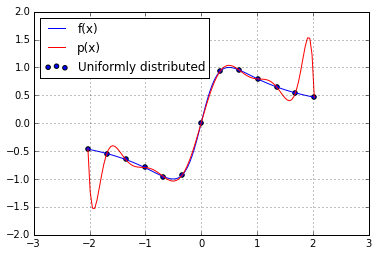
\includegraphics[scale=0.65]{fig1.png}
	\caption{Plot showing the actual and the interpolation by a degree 12 polynomial over uniformly distributed points}
	\label{fig:fig1}
\end{figure}

\begin{figure}[h]
	\center
	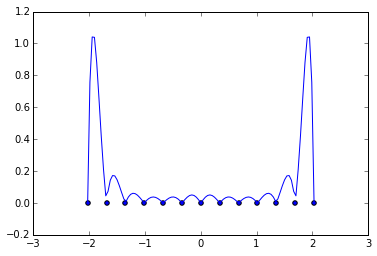
\includegraphics[scale=0.65]{err1.png}
    \caption{The absolute error $|f(x) - p(x)|$ in polynomial interpolation of $\frac{x}{(0.25 + x^2)}$ using 13 equally spaced points.}
	\label{fig:err1}
\end{figure}
	

The corresponding python code can be found at \ref{code:problem3a}
\clearpage

\section{Solution to Question 3 (b)}\label{prob3b}

In this section, we use Chebychev nodes to control the fit of the polynomials at the ends. The red points in \ref{fig:fig2} are the Chebychev nodes and the blue curve is the target function. The red curve is the interpolating curve which can be visually seen to fit the target function better. This can be asserted, since the mean absolute error between the target function and the Chebychev interpolated function is 0.0272302580903 which is significantly lower that the error obtained after interpolating over uniformly distributed points. The only error we get after Interpolating using Chebychev nodes is at the central nodes \ref{fig:err2}, and that too its an order of magnitude lower than the error peaks seen in the absolute error graph when using uniformly distributed nodes in \ref{fig:err1}

\begin{figure}[h]
    \centering
    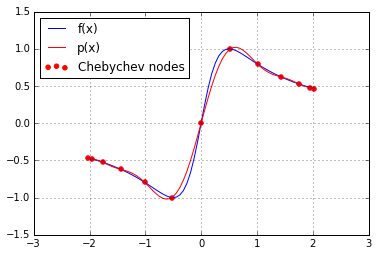
\includegraphics[scale=0.65]{fig2.png}
    \caption{Plot showing the actual and the interpolation by a degree 12 polynomial over Chebychev nodes.}
    \label{fig:fig2}
\end{figure}

\begin{figure}[h]
    \centering
    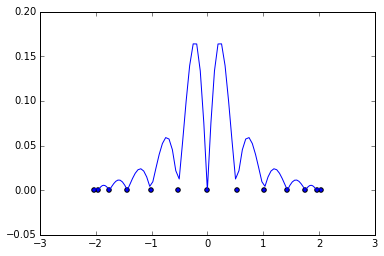
\includegraphics[scale=0.65]{err2.png}
    \caption{The absolute error $|f(x) - p(x)|$ in polynomial interpolation of $\frac{x}{0.25 + x^2}$ using 13 Chebychev nodes.}
    \label{fig:err2}
\end{figure}


The corresponding python code can be found at \ref{code:problem3b}
\clearpage

\clearpage
%\ldots

\clearpage
\section{Appendix A}\label{code:problem3a}
Python source code for \ref{prob3a}.
{\footnotesize
\begin{lstlisting}
import numpy as np
import pylab as pl

# Defining the Target function
f = lambda x: x / ( 0.25 + x*x)

# Interval
xmin, xmax = -2.02857, 2.02857
n_points = 13
n = 12 # order of polynomial to fit
plot_points = 101

# 13 uniformly distributed points
points_uniform = np.linspace(xmin,xmax,n_points)
# Taking a much greater number of points to get a smooth function
points_function_plot = np.linspace(xmin, xmax, plot_points)

def coefficients(n, x, y):
    # n is the degree of the desired polynomial
    #print "x",len(x),"y",len(y) 
    a = y
    for j in range(1,n+1):
        for i in range(n,j-1,-1):
            a[i] = (a[i] - a[i-1]) / (x[i] - x[i-j])
            #print "a", len(a)
    return a

def evaluate(n, x, a, t):
    pt = a[n]
    for i in range(n-1, -1, -1):
        pt = pt * (t - x[i]) + a[i];
    return pt

# Take linearly spaced X and get Y from the polynomial's analytical expression
x,y = points_uniform, f(points_uniform)

# Get Coefficients
coeff = coefficients(n, x, y)

evaluation = np.asarray([evaluate(n, x, coeff, t) for t in x], np.float)
#print evaluation

evaluation_100 = np.asarray([evaluate(n, x, coeff, t) for t in points_function_plot], np.float)
#print evaluation_100

# Plot the 13 points we are interested in.
pl.scatter(points_uniform, f(points_uniform),label="Uniformly distributed")
# Plot the curve.
pl.plot(points_function_plot, f(points_function_plot),label="f(x)")
pl.plot(points_function_plot, evaluation_100, color='red',label="p(x)")
# Turn on grids
pl.grid()
pl.legend(loc="upper left")
#pl.figtext(-0.05,0,"Plot showing the actual and the interpolation by a degree 12 polynomial over uniformly distributed points")
pl.show()

# The mean absolute error
error = np.mean(np.abs(evaluation_100 - f(points_function_plot)))
print error

# 13 uniformly spaced points
pl.scatter(points_uniform, 0 * points_uniform)

#Error
error = np.abs(evaluation_100 - f(points_function_plot))
pl.plot(points_function_plot, error)
\end{lstlisting}
}

\clearpage
\section{Appendix B}\label{code:problem3b}
Python source code for \ref{prob3b}.
{\footnotesize
\begin{lstlisting}
import numpy as np
import pylab as pl

# Defining the Target function
f = lambda x: x / ( 0.25 + x*x)

# Interval
xmin, xmax = -2.02857, 2.02857
n_points = 13
n = 12 # order of polynomial to fit
plot_points = 101

# 13 uniformly distributed points
points_uniform = np.linspace(xmin,xmax,n_points)
# Taking a much greater number of points to get a smooth function
points_function_plot = np.linspace(xmin, xmax, plot_points)

def coefficients(n, x, y):
    # n is the degree of the desired polynomial
    #print "x",len(x),"y",len(y) 
    a = y
    for j in range(1,n+1):
        for i in range(n,j-1,-1):
            a[i] = (a[i] - a[i-1]) / (x[i] - x[i-j])
            #print "a", len(a)
    return a

def evaluate(n, x, a, t):
    pt = a[n]
    for i in range(n-1, -1, -1):
        pt = pt * (t - x[i]) + a[i];
    return pt


def get_chebychev(n,a,b):
    '''
    A closure which returns a function which would return
    chebychev nodes for n number of points in the interval [a,b]
    '''
    def chebychev(i):
        return 0.5*(a+b) + 0.5*(b-a)*np.cos((i*np.pi)/n)
    return chebychev

# Chebychev nodes for n_points=13
chebychev = get_chebychev(n_points-1,xmin, xmax) 
# range(n) => [0,n-1]
chebychev_nodes = np.asarray([chebychev(i) for i in range(n_points)], np.float) 

#Chebychev nodes for plot_points=100 points
chebychev = get_chebychev(plot_points-1,xmin, xmax) 
# range(n+1) => [0,n]
chebychev_nodes_100 = np.asarray([chebychev(i) for i in range(plot_points)], np.float) 

#Check to ensure the 7th Chebychev node is 0
for idx, node in enumerate(chebychev_nodes):
    print idx, node

y = f(chebychev_nodes)
x = chebychev_nodes
# Get coefficients for Chebychev Nodes
coeff = coefficients(n, x, y)

cheby_eval = np.asarray(
                    [evaluate(n, chebychev_nodes, coeff, t) for t in chebychev_nodes]
                    , np.float)
cheby_eval_100 = np.asarray(
                    [evaluate(n, chebychev_nodes, coeff, t) for t in chebychev_nodes_100]
                    , np.float)

# Plot the 13 Chebychev points we are interested in.
pl.scatter(chebychev_nodes, cheby_eval, color='red', label="Chebychev nodes")

# Plot the curve.
pl.plot(chebychev_nodes_100, f(chebychev_nodes_100),label="f(x)")
pl.plot(chebychev_nodes_100, cheby_eval_100, color='red',label="p(x)")
# Turn on grids
pl.legend(loc="upper left")
pl.grid()
pl.show()

error = np.mean(np.abs(cheby_eval_100 - f(chebychev_nodes_100)))
print error

# 13 chebychev points
pl.scatter(chebychev_nodes, 0 * chebychev_nodes)

#Error
error = np.abs(cheby_eval_100 - f(chebychev_nodes_100))
pl.plot(chebychev_nodes_100, error)
pl.show()

\end{lstlisting}
}

\end{document}

